% ================================================================
\section{Đặt vấn đề hình thức}
\label{sec:formal-problem}

Bài toán tổng hợp ảnh y tế đa phương thức được định nghĩa như sau. Cho hai ảnh nguồn $I_V, I_I \in \mathbb{R}^{H \times W}$ từ hai phương thức khác nhau (ví dụ $I_V$ là MRI, $I_I$ là CT), cần tìm ảnh tổng hợp $F \in \mathbb{R}^{H \times W}$ thỏa mãn hai ràng buộc đồng thời:
\begin{enumerate}\itemsep2pt
    \item Bảo toàn cấu trúc: $F$ phải giữ lại thông tin cấu trúc giải phẫu chung từ cả hai modality, phản ánh qua các chỉ số cường độ (SSIM, PSNR, MI).
    \item Bảo toàn chi tiết: $F$ phải giữ lại các cạnh và texture đặc thù từng modality, phản ánh qua các chỉ số tần số không gian (SF, AG, EI, Qabf).
\end{enumerate}

Trong kiến trúc CDDFuse, hai ràng buộc này được xử lý qua hai luồng song song trong Fusion Layer. Gọi $\Phi_{\mathrm{enc}}$ là Encoder dùng chung trọng số, với đầu ra:
\begin{align}
(f_V^B,\, f_V^D) &= \Phi_{\mathrm{enc}}(I_V) \\
(f_I^B,\, f_I^D) &= \Phi_{\mathrm{enc}}(I_I)
\end{align}
trong đó $f^B \in \mathbb{R}^{H' \times W' \times C}$ là đặc trưng Base (tần số thấp, tương quan cao) và $f^D \in \mathbb{R}^{H' \times W' \times C}$ là đặc trưng Detail (tần số cao, tương quan thấp). Quá trình tổng hợp được thực hiện độc lập trên hai nhánh:
\begin{align}
f_F^B &= \Psi_B\!\left(R_B(f_V^B,\, f_I^B)\right) \\
f_F^D &= \Psi_D\!\left(R_D(f_V^D,\, f_I^D)\right)
\end{align}
trong đó $R_B, R_D$ là quy tắc tiền tổng hợp và $\Psi_B, \Psi_D$ là BaseFuseLayer và DetailFuseLayer. Ảnh đầu ra được tái tạo bởi Decoder $\Phi_{\mathrm{dec}}$:
\begin{equation}
F = \Phi_{\mathrm{dec}}\!\left(\mathrm{Conv}_{1\times1}\!\left(\mathrm{cat}(f_F^B,\, f_F^D)\right)\right)
\end{equation}

CDDFuse gốc dùng $R_B = R_D = \text{Sum}$ (phép cộng). Đồ án đề xuất thay bằng $R_B = R_{\mathrm{WAvg}}$ và $R_D = R_{\mathrm{SML}}$, giữ nguyên toàn bộ $\Phi_{\mathrm{enc}}$, $\Psi_B$, $\Psi_D$, $\Phi_{\mathrm{dec}}$.

% ================================================================
\section{Kiến trúc CDDFuse-AG}
\label{sec:cddfuse-ag-arch}

Mô hình đề xuất \textbf{CDDFuse-AG} (Asymmetric Gating) giữ nguyên kiến trúc CDDFuse, chỉ thay thế phép cộng ở Fusion Layer bằng hai quy tắc bất đối xứng:

\begin{align}
f_F^B &= \mathrm{BaseFuseLayer}\!\left(R_{\mathrm{WAvg}}(f_V^B,\; f_I^B)\right) \label{eq:ag-base} \\
f_F^D &= \mathrm{DetailFuseLayer}\!\left(R_{\mathrm{SML}}(f_V^D,\; f_I^D)\right) \label{eq:ag-detail}
\end{align}

trong đó $R_{\mathrm{WAvg}}$ là quy tắc trung bình có trọng số học được cho nhánh Base, và $R_{\mathrm{SML}}$ là quy tắc lựa chọn theo Sum-Modified-Laplacian cho nhánh Detail (định nghĩa chi tiết tại Mục~\ref{sec:proposed-rules}).

\paragraph{Channel Reduction.}
Hai đặc trưng $f_F^B$ và $f_F^D$ (mỗi cái $64$ kênh) được nối kênh rồi chiếu về $64$ kênh bằng Conv$_{1\times1}$ trước khi đưa vào Decoder:
\begin{equation}
f_{\mathrm{merge}} = \mathrm{Conv}_{1\times1}\!\left(\mathrm{cat}(f_F^B,\; f_F^D)\right), \quad 128\!\to\!64 \text{ kênh}
\end{equation}

\begin{figure}[H]
\centering
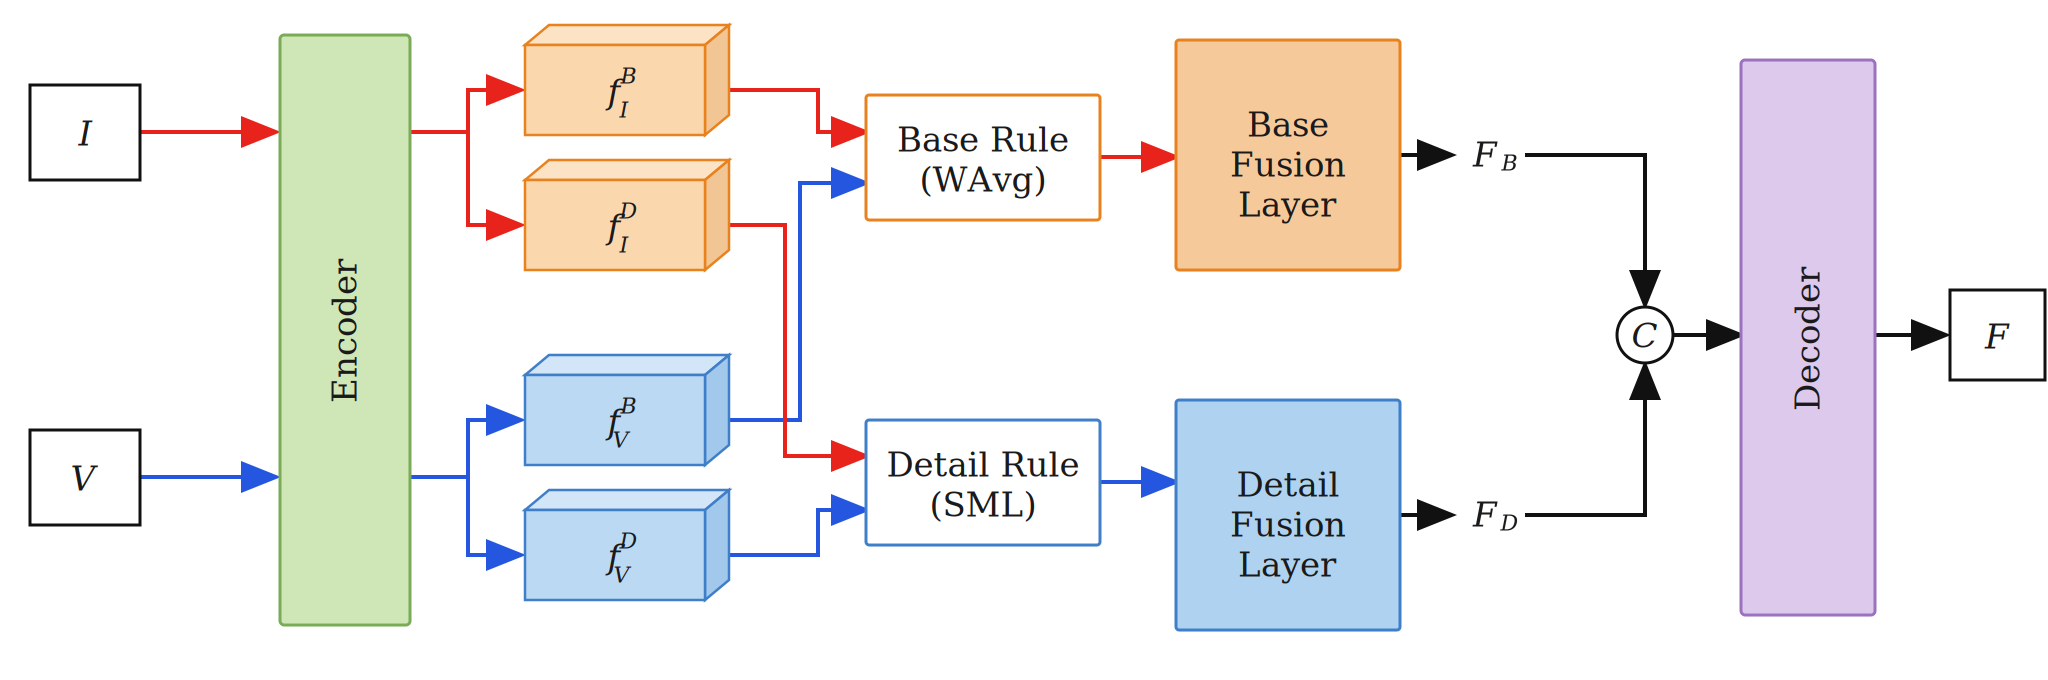
\includegraphics[width=0.97\textwidth]{figures/fusion_diagram_cddag.png}
\caption{Kiến trúc CDDFuse-AG: Encoder dùng chung trọng số trích xuất đặc trưng Base/Detail, Fusion Layer áp dụng bất đối xứng (WAvg cho Base, SML cho Detail), Decoder tái tạo ảnh tổng hợp $F$.}
\label{fig:cddfuse-ag-arch}
\end{figure}

\paragraph{Tổng số tham số.}
\begin{center}
\setlength{\tabcolsep}{8pt}
\begin{tabular}{lrr}
\toprule
\textbf{Thành phần} & \textbf{Kiến trúc} & \textbf{Số tham số} \\
\midrule
Encoder                         & PatchEmbed + 4$\times$TransBlock + BFE + DFE$_3$ & $599{,}144$ \\
\quad patch\_embed              & Conv$3\!\times\!3$, $1\!\to\!64$                  & $576$ \\
\quad encoder\_level1           & $4\times$ TransformerBlock, $\mathrm{dim}=64$     & $181{,}024$ \\
\quad baseFeature               & BaseFeatureExtraction, $\mathrm{heads}=8$         & $363{,}016$ \\
\quad detailFeature             & DetailFeatureExtraction, $3\times$ DetailNode     & $54{,}528$ \\
\midrule
BaseFuseLayer                   & BaseFeatureExtraction, $\mathrm{dim}=64$          & $363{,}016$ \\
DetailFuseLayer                 & DetailFeatureExtraction, $1\times$ DetailNode     & $18{,}176$ \\
\midrule
Decoder                         & ReduceChannel + 4$\times$TransBlock + Output      & $207{,}936$ \\
\quad reduce\_channel           & Conv$1\!\times\!1$, $128\!\to\!64$               & $8{,}192$ \\
\quad encoder\_level2           & $4\times$ TransformerBlock, $\mathrm{dim}=64$     & $181{,}024$ \\
\quad output                    & Conv$3\!\times\!3 \to$ LeakyReLU $\to$ Conv$3\!\times\!3$ & $18{,}720$ \\
\midrule
\textbf{Quy tắc WAvg} (Base)   & scalar $\theta \in \mathbb{R}$                    & \textbf{1} \\
\textbf{Quy tắc SML} (Detail)  & refine Conv$1\!\times\!1$, $64\!\to\!64$         & $4{,}160$ \\
\midrule
\textbf{Tổng tham số}          &                                                   & $\mathbf{1{,}192{,}433}$ \\
\bottomrule
\end{tabular}
\end{center}

So với CDDFuse baseline ($1{,}188{,}272$ tham số), CDDFuse-AG chỉ thêm \textbf{4{,}161 tham số} ($\approx 0{,}35\%$) từ WAvg ($\theta$) và SML refine Conv. Toàn bộ tham số được huấn luyện end-to-end; Encoder dùng chung trọng số (shared weights) cho cả hai modality đầu vào.

% ================================================================
\section{Phân tích điểm can thiệp}
\label{sec:intervention}

Kiến trúc CDDFuse gồm ba khối tuần tự: Encoder $\to$ Fusion Layer $\to$ Decoder (Mục~\ref{ssec:cddfuse-arch}). Encoder và Decoder đã được tối ưu hóa để phân rã và tái tạo ảnh một cách ổn định. Điểm can thiệp duy nhất của đề xuất là Fusion Layer --- cụ thể là phép cộng $f_I + f_V$ được dùng mặc định ở đầu mỗi nhánh trước BaseFuseLayer và DetailFuseLayer.

\subsection{Vì sao phép cộng Sum làm giảm chất lượng chi tiết}
\label{ssec:sum-analysis}

Xét hai đặc trưng Detail $f_V^D$ và $f_I^D$ tại một vị trí không gian $(i,j)$ cụ thể. Giả sử modality $V$ (MRI) có cạnh sắc nét tại đó --- tức $|f_V^D|_{ij} \gg |f_I^D|_{ij}$ --- trong khi modality $I$ (CT) không có cạnh tương ứng. Phép cộng Sum cho ra:
\begin{equation}
(f_V^D + f_I^D)_{ij} = f_{V,ij}^D + f_{I,ij}^D
\end{equation}
Vì $f_{I,ij}^D$ mang nhiễu nền hoặc thông tin không liên quan đến cạnh tại vị trí đó, tổng thu được sẽ sai lệch so với giá trị gốc $f_{V,ij}^D$. Quan trọng hơn, hệ số nhân bằng $1$ cho cả hai modality nghĩa là CT ``pha loãng'' thông tin cạnh MRI một cách không có kiểm soát. Nếu $f_{I,ij}^D$ ngẫu nhiên trái dấu với $f_{V,ij}^D$, cạnh MRI bị triệt tiêu một phần.

Ngược lại, quy tắc SML tính trọng số $w_a$ dựa trên độ sắc nét cục bộ: nếu MRI có cạnh mạnh hơn CT tại $(i,j)$, thì $w_a \approx 1$ và kết quả tổng hợp xấp xỉ $2 f_{V,ij}^D$ --- giữ nguyên cạnh MRI mà không bị pha loãng bởi CT.

Phân tích tần số lượng hóa điều này: phép cộng hai tín hiệu $s_V$ và $s_I$ tại miền tần số tương đương với:
\begin{equation}
\mathcal{F}(s_V + s_I) = \mathcal{F}(s_V) + \mathcal{F}(s_I)
\end{equation}
Năng lượng tần số cao trong $\mathcal{F}(s_V + s_I)$ phụ thuộc vào pha tương đối giữa hai tín hiệu. Nếu hai modality có cạnh không cùng pha (điều phổ biến trong CT--MRI do cơ chế vật lý khác nhau), cộng tuyến tính khuếch đại một số tần số nhưng triệt tiêu số khác --- kết quả không dự đoán được và phụ thuộc vào từng cặp ảnh cụ thể. Ngược lại, SML lựa chọn dựa trên biên độ cục bộ, không bị ảnh hưởng bởi thông tin pha.

\subsection{Lý do chỉ can thiệp tại Fusion Layer}
\label{ssec:why-fusion-layer}

Đề xuất của đồ án giữ nguyên toàn bộ Encoder và Decoder, chỉ thay thế quy tắc tiền tổng hợp $R_B$ và $R_D$. Lựa chọn này có ba lý do:

\begin{itemize}\itemsep2pt
    \item So sánh công bằng: mọi sai biệt kết quả đến trực tiếp từ quy tắc tổng hợp, loại bỏ ảnh hưởng của kiến trúc encoder/decoder.
    \item Tận dụng pretrained weights: CDDFuse đã được huấn luyện hội tụ trên tập Harvard MIF; khởi tạo từ checkpoint này giúp CDDFuse-AG hội tụ nhanh hơn đáng kể so với train từ đầu.
    \item Kiểm soát số tham số: toàn bộ đóng góp mới chỉ là \textbf{4.161 tham số}, cho phép kết luận rõ ràng rằng cải thiện đến từ thiết kế quy tắc, không phải từ tăng dung lượng mô hình.
\end{itemize}

% ================================================================
\section{Nguyên lý thiết kế bất đối xứng}
\label{sec:asymmetric-principle}

CDDFuse phân rã ảnh thành hai thành phần với bản chất hoàn toàn khác nhau (Hình~\ref{fig:asymmetric-principle}):

\begin{itemize}\itemsep0pt
    \item Nhánh Base (tần số thấp): mang thông tin cấu trúc giải phẫu chung, tương quan cao giữa hai modality. Hai modality thường đồng thuận ở mức độ toàn cục --- MRI và CT đều thể hiện cùng cơ quan, cùng vị trí giải phẫu.
    \item Nhánh Detail (tần số cao): mang texture, cạnh và thông tin đặc thù của từng modality. CT nổi bật về cấu trúc xương cứng; MRI nổi bật về mô mềm. Hai nguồn mang thông tin bổ sung nhau chứ không đồng thuận.
\end{itemize}

Từ sự khác biệt bản chất này, Liu et al.\ \cite{liu2018survey} đề xuất nguyên tắc:
\begin{center}
\emph{``Base cần trung bình hóa (averaging) --- Detail cần lựa chọn theo hoạt động cục bộ (activity-based selection).''}
\end{center}

Phép cộng Sum của CDDFuse gốc áp dụng cùng một chiến lược cho cả hai nhánh, không khai thác được sự khác biệt này. Đề xuất CDDFuse-AG áp dụng hai quy tắc khác nhau cho hai nhánh --- thiết kế \emph{bất đối xứng} (\emph{asymmetric}).

\begin{figure}[H]
\centering
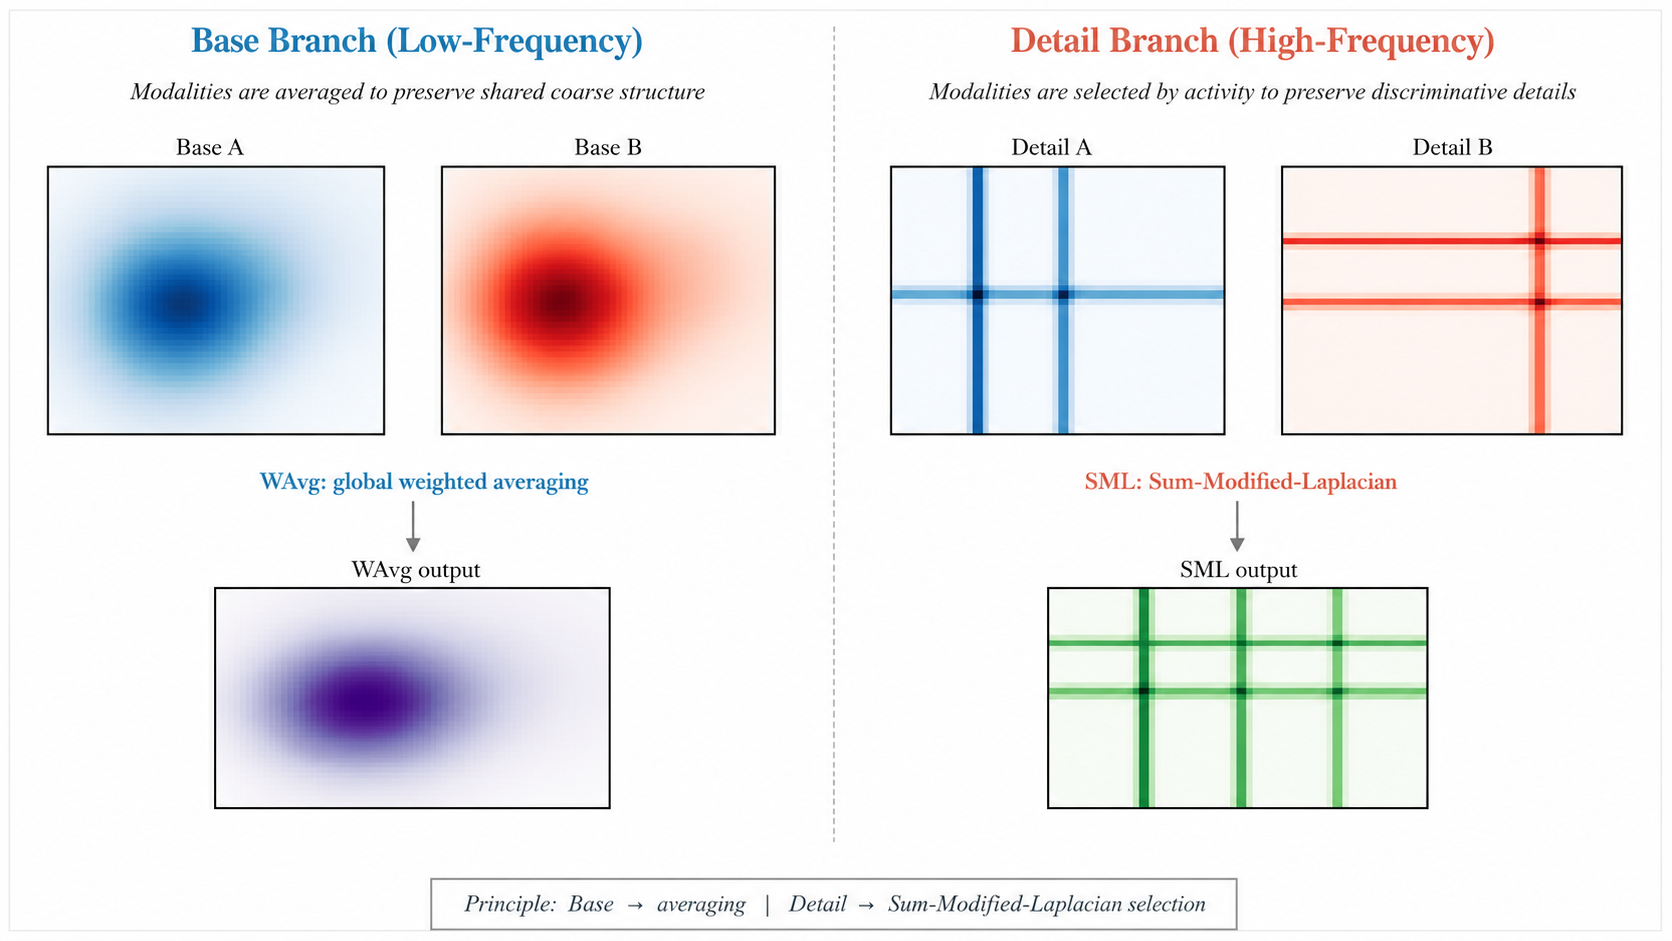
\includegraphics[width=0.96\textwidth]{figures/fig_asymmetric_principle.png}
\caption{Nguyên lý bất đối xứng: nhánh Base (tần số thấp, đồng thuận) phù hợp với trung bình hóa WAvg; nhánh Detail (tần số cao, bổ trợ) phù hợp với lựa chọn theo độ sắc nét SML. (Hình tự thiết kế)}
\label{fig:asymmetric-principle}
\end{figure}

% ================================================================
\section{Quy tắc tổng hợp đề xuất}
\label{sec:proposed-rules}

\subsection{Quy tắc Base: Weighted Average Scalar (WAvg)}
\label{ssec:rule-wavg}

Nhánh Base cần trung bình hóa thông tin cấu trúc chung của hai modality. Thay vì phép cộng cố định, đề xuất dùng trung bình có trọng số học được. Ý tưởng trung bình hóa có trọng số được sử dụng rộng rãi trong các phương pháp fusion truyền thống~\cite{li2018densefuse, xu2020u2fusion}; ở đây chúng tôi đơn giản hóa thành \emph{một tham số scalar duy nhất} để phù hợp với kiến trúc CDDFuse:

\begin{equation}
\alpha = \sigma(\theta), \quad \theta \in \mathbb{R} \text{ (tham số học duy nhất)}
\end{equation}
\begin{equation}
R_{\mathrm{WAvg}}(a, b) = 2\bigl(\alpha \cdot a + (1-\alpha) \cdot b\bigr)
\label{eq:wavg}
\end{equation}

trong đó $a = f_V^B$, $b = f_I^B$ là đặc trưng Base của hai modality, $\sigma$ là hàm sigmoid đảm bảo $\alpha \in (0,1)$, và hệ số $2$ chuẩn hóa để giữ nguyên biên độ so với phép cộng gốc. Tham số $\theta$ khởi tạo bằng $0$ ($\alpha = 0{,}5$) và được học qua huấn luyện Phase~II.

\begin{figure}[H]
\centering
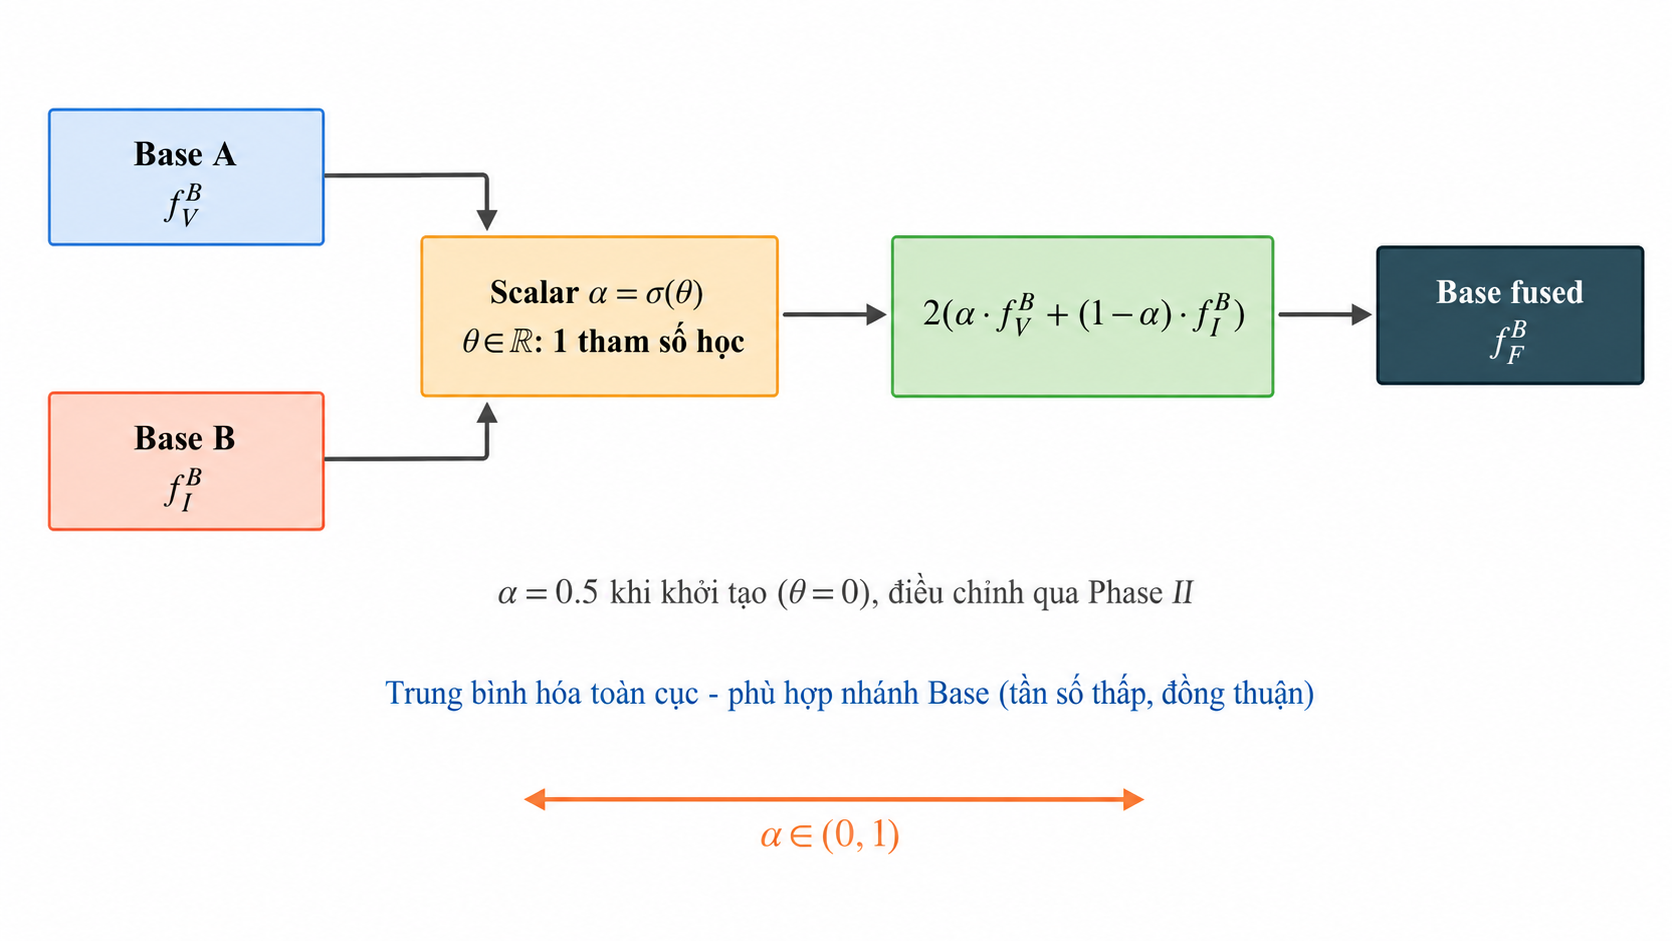
\includegraphics[width=0.88\textwidth]{figures/fig_rule_wavg.png}
\caption{Quy tắc Weighted Average (WAvg) cho nhánh Base: hai feature map Base A và B được kết hợp bằng trọng số scalar $\alpha$ học được, đảm bảo trung bình hóa toàn cục có thể điều chỉnh. (Hình tự thiết kế)}
\label{fig:rule-wavg}
\end{figure}

\paragraph{Lý do chọn WAvg cho nhánh Base.}
\begin{itemize}\itemsep0pt
    \item Chỉ 1 tham số học: tránh overfitting và không phá vỡ phân phối đặc trưng mà Encoder đã học.
    \item Trung bình hóa toàn cục: phù hợp với bản chất đồng thuận của Base --- không cần phân biệt theo vị trí không gian.
    \item Trọng số tối ưu cho từng modality: thay vì giả định $\alpha = 0{,}5$ cố định, mô hình tự học tỷ lệ đóng góp tối ưu giữa hai nguồn.
\end{itemize}

\subsection{Quy tắc Detail: Sum-Modified-Laplacian (SML)}
\label{ssec:rule-sml}

Nhánh Detail cần lựa chọn, tại từng vị trí không gian, modality nào cung cấp thông tin chi tiết (cạnh, texture) phong phú hơn. Đề xuất dùng Sum-Modified-Laplacian (SML) làm thước đo độ sắc nét cục bộ. SML được đề xuất bởi Huang và Jing~\cite{huang2007sml} trong bối cảnh đánh giá độ nét cho multi-focus fusion; ở đây chúng tôi áp dụng vào bài toán multi-modal fusion để đo hoạt động chi tiết trên từng kênh đặc trưng:

\begin{equation}
\mathrm{ML}_{ij}(f) = |2f_{ij} - f_{i-1,j} - f_{i+1,j}| + |2f_{ij} - f_{i,j-1} - f_{i,j+1}|
\label{eq:ml}
\end{equation}
\begin{equation}
\mathrm{SML}_{ij}(f) = \sum_{(p,q) \in \mathcal{N}(i,j)} \mathrm{ML}_{pq}(f)
\label{eq:sml}
\end{equation}

trong đó $\mathcal{N}(i,j)$ là vùng lân cận $3\times 3$ quanh pixel $(i,j)$. SML tích lũy năng lượng Laplacian hiệu chỉnh (Modified Laplacian) trong vùng lân cận, đo mức độ ``sắc nét'' hay ``hoạt động chi tiết'' tại từng điểm.

Dựa trên SML, trọng số tổng hợp theo vị trí được tính:
\begin{equation}
w_a = \frac{\mathrm{SML}(a)}{\mathrm{SML}(a) + \mathrm{SML}(b) + \epsilon}
\end{equation}
\begin{equation}
R_{\mathrm{SML}}(a, b) = 2\bigl(w_a \odot a + (1 - w_a) \odot b\bigr)
\label{eq:sml-rule}
\end{equation}

trong đó $a = f_V^D$, $b = f_I^D$ là đặc trưng Detail, $\epsilon$ là hằng số ổn định số học, $\odot$ là phép nhân từng phần tử.

\begin{figure}[H]
\centering
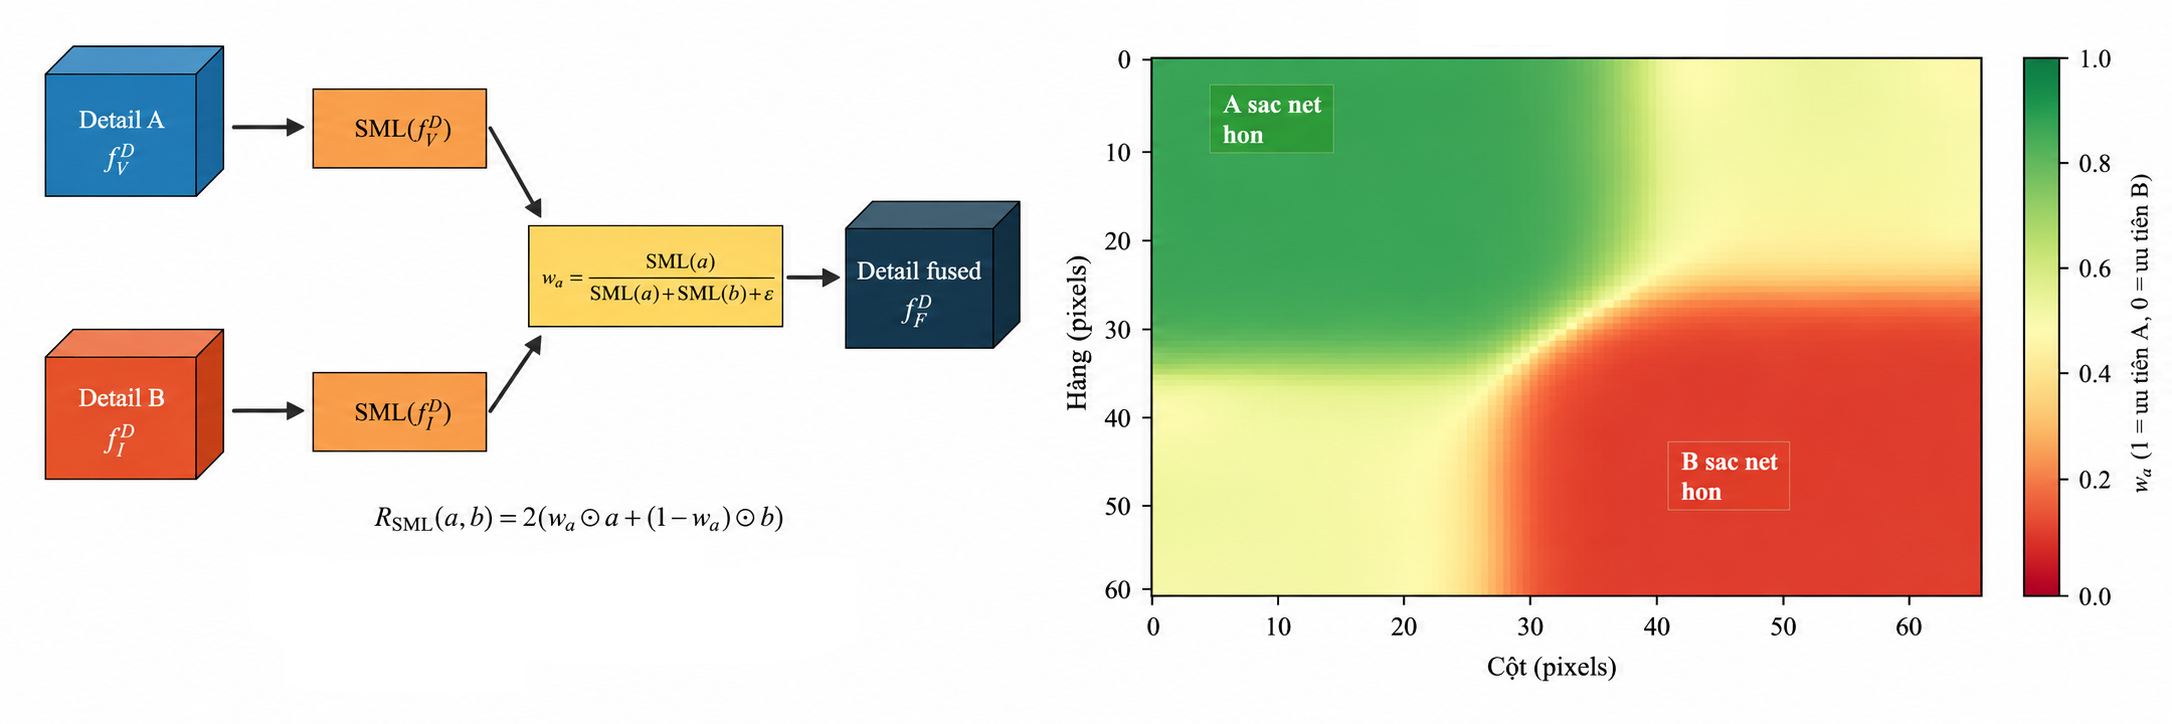
\includegraphics[width=0.95\textwidth]{figures/fig_rule_sml.png}
\caption[Quy tắc SML cho nhánh Detail]{Quy tắc SML cho nhánh Detail: (trái) sơ đồ tính weight map từ SML của hai feature map; (phải) ví dụ weight map $w_a$ --- vùng xanh lá ưu tiên Detail A, vùng đỏ ưu tiên Detail B theo độ sắc nét cục bộ. (Hình tự thiết kế; công thức SML từ~\cite{huang2007sml})}
\label{fig:rule-sml}
\end{figure}

\paragraph{Lý do chọn SML cho nhánh Detail.}
\begin{itemize}\itemsep0pt
    \item Nhạy với cạnh và tần số cao: Modified Laplacian đặc biệt nhạy với các biến thiên đột ngột --- đúng với bản chất tần số cao của nhánh Detail.
    \item Lựa chọn theo vị trí (spatially adaptive): tại mỗi điểm ảnh, modality nào có cạnh sắc nét hơn sẽ được ưu tiên --- khai thác tính bổ trợ giữa MRI (mô mềm) và CT/PET/SPECT (cấu trúc đặc thù).
    \item Không có tham số học: quy tắc hoàn toàn dựa trên đặc trưng đầu vào, không phụ thuộc vào khởi tạo hay dữ liệu huấn luyện --- tính tổng quát hóa cao.
\end{itemize}

% ================================================================
\section{Phân tích tham số WAvg và ý nghĩa lâm sàng}
\label{sec:wavg-analysis}

\subsection{Ý nghĩa của tham số $\alpha$}
\label{ssec:alpha-meaning}

Tham số duy nhất của quy tắc WAvg là $\theta \in \mathbb{R}$, được chuyển sang $\alpha = \sigma(\theta) \in (0,1)$ qua hàm sigmoid. Sau khi huấn luyện hội tụ, $\alpha$ phản ánh tỷ lệ đóng góp tối ưu giữa hai modality cho thành phần cấu trúc tổng thể:

\begin{itemize}\itemsep2pt
    \item $\alpha > 0{,}5$: mô hình đặt trọng số cao hơn cho modality $V$ (MRI) trong thành phần Base --- hợp lý khi MRI cung cấp cấu trúc mô mềm chi tiết hơn CT/PET/SPECT cho hầu hết vùng não.
    \item $\alpha < 0{,}5$: mô hình ưu tiên modality $I$ (CT/PET/SPECT) --- xảy ra khi thành phần tần số thấp của nguồn thứ hai mang nhiều thông tin cấu trúc hơn.
    \item $\alpha = 0{,}5$: tương đương phép cộng Sum gốc (sau khi chia 2) --- tức CDDFuse gốc là trường hợp đặc biệt của CDDFuse-AG với $\theta = 0$.
\end{itemize}

Điều này có ý nghĩa lâm sàng trực tiếp: mô hình tự học được modality nào cần được ưu tiên cho thành phần cấu trúc trên tập dữ liệu cụ thể, thay vì lập trình cứng tỷ lệ $50\text{--}50$.

\subsection{Khởi tạo và hội tụ}
\label{ssec:alpha-convergence}

$\theta$ được khởi tạo bằng $0$ ($\alpha_0 = 0{,}5$), đảm bảo điểm xuất phát là phép cộng đối xứng --- tương tự CDDFuse gốc. Trong Pha~I (đóng băng WAvg), $\theta$ không thay đổi. Trong Pha~II (huấn luyện end-to-end), gradient từ hàm mất mát $\mathcal{L}_{\mathrm{int}}$ và $\mathcal{L}_{\mathrm{grad}}$ điều chỉnh $\theta$ để tối ưu hóa chất lượng ảnh tổng hợp trên tập huấn luyện Harvard MIF.

Vì WAvg chỉ có một bậc tự do và $\sigma(\cdot)$ liên tục, gradient luôn tồn tại và $\alpha$ hội tụ nhanh mà không gây bất ổn định quá trình huấn luyện --- đây là lợi thế so với các quy tắc Base phức tạp hơn (VSM, LocalEnergy) đòi hỏi tính toán nặng hơn và dễ gây bất ổn khi tích hợp vào pipeline end-to-end.

% ================================================================
\section{Phân tích độ phức tạp tính toán}
\label{sec:complexity}

So với CDDFuse gốc, CDDFuse-AG chỉ thêm hai thao tác nhỏ tại Fusion Layer trong quá trình suy diễn (inference):

\begin{enumerate}\itemsep2pt
    \item Tính WAvg cho nhánh Base: một phép nhân vô hướng và cộng vector --- chi phí $O(H'W'C)$, không đáng kể so với BaseFuseLayer ($O(H'W'C^2)$ với self-attention).
    \item Tính SML cho nhánh Detail: tính Modified Laplacian qua tích chập $3\times3$ và tổng hợp vùng lân cận $3\times3$ --- chi phí $O(H'W'C)$ với hằng số nhỏ (hai phép tích chập $3\times3$ với kernel cố định).
\end{enumerate}

Bảng~\ref{tab:complexity} tóm tắt so sánh giữa CDDFuse và CDDFuse-AG:

\begin{table}[H]
\centering
\small
\caption{So sánh số tham số và overhead tính toán giữa CDDFuse và CDDFuse-AG.}
\label{tab:complexity}
\setlength{\tabcolsep}{10pt}
\begin{tabular}{lcc}
\toprule
& CDDFuse & CDDFuse-AG \\
\midrule
Tổng tham số & $1{,}188{,}272$ & $1{,}192{,}433$ \\
Tham số thêm & --- & $4{,}161$ ($+0{,}35\%$) \\
Overhead WAvg & --- & $O(H'W'C)$, 1 phép nhân \\
Overhead SML & --- & $O(H'W'C)$, 2 tích chập $3{\times}3$ cố định \\
Thời gian inference & $t_0$ & $t_0 + \Delta t \approx t_0$ \\
\bottomrule
\end{tabular}
\end{table}

Overhead thực tế của SML là không đáng kể vì kernel $3\times3$ với hệ số cố định $[0, -1, 0; -1, 4, -1; 0, -1, 0]$ được thực hiện song song trên GPU trong một lần forward pass. Toàn bộ cải thiện chất lượng đến từ chiến lược lựa chọn thông tin, không phải từ tăng dung lượng mô hình hay chi phí tính toán.
